\documentclass{article}
\usepackage{tikz}
\usetikzlibrary{patterns}

\begin{document}



\begin{figure}
  \begin{minipage}[b]{.46\linewidth}
    \centering 
    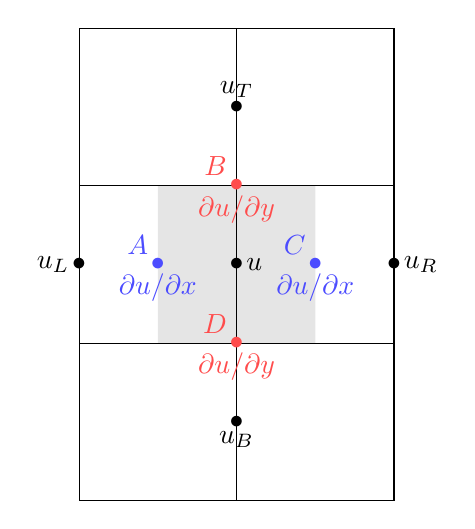
\begin{tikzpicture}

      %% \node[align=center,font=\bfseries, yshift=2em] (title)   at (current bounding box.north) {Fig.1 - Inside the domain};
      %% \draw (title);
      
      % countour du domaine
      % 2 elements suivant X
      % 3 elements suivant Y
      % dx = 2
      % dy = 2
      \draw(0, 0) -- (4, 0);
      \draw(4, 0) -- (4, 6);
      \draw(4, 6) -- (0, 6);
      \draw(0, 6) -- (0, 0);

      % volume de controle
      %% \fill[color=gray!20, pattern=north east lines]
      \fill[color=gray!20] (1, 2) -- (3, 2) -- (3, 4) -- (1, 4) -- (1, 2);

      % lignes horizontales
      \draw(0, 2) -- (4, 2);
      \draw(0, 4) -- (4, 4);

      % ligne verticale
      \draw(2, 0) -- (2, 6);

      % localisation des inconnues
      \node (u) at (2, 3) [right]  {$u$};
      \node (ur) at (4, 3) [right]  {$u_R$};
      \node (ul) at (0, 3) [left]  {$u_L$};
      \node (ut) at (2, 5) [above]  {$u_T$};
      \node (ub) at (2, 1) [below]  {$u_B$};
      \node (ptu) at (2, 3)  {$\bullet$};
      \node (ptur) at (4, 3)  {$\bullet$};
      \node (ptul) at (0, 3)  {$\bullet$};
      \node (ptut) at (2, 5)  {$\bullet$};
      \node (ptub) at (2, 1)  {$\bullet$};

      % localisation des derivees
      \node [color=blue!70] at (1, 3) [below]  {$\partial u/\partial x$};
      \node [color=blue!70] at (1, 3) [above left]  {$A$};
      \node [color=blue!70] at (1, 3)  {$\bullet$};
      \node [color=blue!70] at (3, 3) [below]  {$\partial u/\partial x$};
      \node [color=blue!70] at (3, 3) [above left]  {$C$};
      \node [color=blue!70] at (3, 3)  {$\bullet$};
      \node [color=red!70]  at (2, 4) [below]  {$\partial u/\partial y$};
      \node [color=red!70]  at (2, 4) [above left]  {$B$};
      \node [color=red!70]  at (2, 4)  {$\bullet$};
      \node [color=red!70]  at (2, 2) [below]  {$\partial u/\partial y$};
      \node [color=red!70]  at (2, 2) [above left]  {$D$};
      \node [color=red!70]  at (2, 2)  {$\bullet$};  
    \end{tikzpicture}    
    \caption{Inside the domain.}
  \end{minipage} \hfill 
  \begin{minipage}[b]{.46\linewidth}
    \centering

    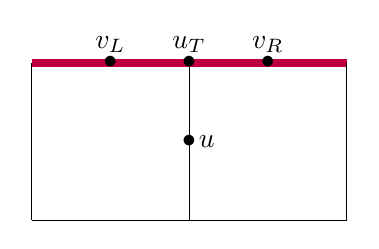
\begin{tikzpicture}
      
      %bordure 
      \draw [color=purple, thick, line width=1mm] (0,2) -- (4,2);
      %lignes verticales
      \draw(2,0)--(2,2);
      \draw(0,0)--(0,2);
      \draw(4,0)--(4,2);
      %ligne horizontale
      \draw(0,0)--(4,0);

      \node at (1, 2) [above] {$v_L$};    
      \node at (1, 2) {$\bullet$};    
      \node at (2, 2) [above] {$u_T$};
      \node at (2, 2) {$\bullet$};    
      \node at (3, 2) [above] {$v_R$};
      \node at (3, 2) {$\bullet$};
      \node at (2, 1) [right] {$u$};
      \node at (2, 1) {$\bullet$};
    \end{tikzpicture}

    \caption{Zoom on a top boundary.}
  \end{minipage} \hfill
  \begin{minipage}[b]{.90\linewidth}
    \centering

    \begin{tikzpicture}
      
      %bordure 
      \draw(0,0) -- (0,4) -- (4,4) -- (4,2) -- (2,2) -- (2,0) --(0,0) ;
      %lignes internes
      \draw(0,2)--(2,2);
      \draw(2,2)--(2,4);

      \node at (0, 1) {$\bullet$};    
      \node at (0, 1) [left] {$u_1$};
      \node at (0, 3) {$\bullet$};    
      \node at (0, 3) [left] {$u_0$};
      \node at (1, 4) {$\bullet$};    
      \node at (1, 4) [above] {$v_0$};
      \node at (3, 4) {$\bullet$};    
      \node at (3, 4) [above] {$v_1$};

      \node [ line width=0.8mm, fill=purple, circle] at (0,4) {};
    \end{tikzpicture}

    \caption{Zoom on a left top corner.}
  \end{minipage}
\end{figure}



\end{document}

